%-------------------------
% Report: local coding agent on SWE-bench Verified
% Bilal Rana
% Layout follows the Jake Gutierrez (MIT) template used for the CV
% Build: tectonic report_latex.tex   (needs architecture.pdf: rsvg-convert -f pdf -o architecture.pdf architecture.svg)
%------------------------

\documentclass[letterpaper,11pt]{article}

\usepackage{latexsym}
\usepackage[empty]{fullpage}
\usepackage{titlesec}
\usepackage[usenames,dvipsnames]{color}
\usepackage{enumitem}
\usepackage[hidelinks]{hyperref}
\usepackage{fancyhdr}
\usepackage[english]{babel}
\usepackage{tabularx}
\usepackage{booktabs}
\usepackage{graphicx}
\usepackage{needspace}
\usepackage{iftex}
\ifPDFTeX\input{glyphtounicode}\fi

\pagestyle{fancy}
\fancyhf{} % clear all header and footer fields
\fancyfoot{}
\renewcommand{\headrulewidth}{0pt}
\renewcommand{\footrulewidth}{0pt}

% Adjust margins
\addtolength{\oddsidemargin}{-0.5in}
\addtolength{\evensidemargin}{-0.5in}
\addtolength{\textwidth}{1in}
\addtolength{\topmargin}{-.5in}
\addtolength{\textheight}{1.45in}

\urlstyle{same}

\raggedbottom
\raggedright
\setlength{\tabcolsep}{0in}

% Sections formatting
\titleformat{\section}{
  \vspace{-7pt}\scshape\raggedright\large
}{}{0em}{}[\color{black}\titlerule \vspace{-6pt}]

% Ensure that generated pdf is machine readable (pdfLaTeX only; XeTeX does this itself)
\ifPDFTeX\pdfgentounicode=1\fi

%-------------------------
% Custom commands
\newcommand{\resumeItem}[1]{
  \item\small{
    {#1 \vspace{-2pt}}
  }
}

\newcommand{\resumeItemListStart}{\begin{itemize}[leftmargin=0.15in, label={}]}
\newcommand{\resumeItemListEnd}{\end{itemize}\vspace{-5pt}}
\newcommand{\bulletListStart}{\begin{itemize}[leftmargin=0.3in, itemsep=1pt, parsep=0pt, topsep=2pt]}
\newcommand{\bulletListEnd}{\end{itemize}\vspace{-3pt}}

\newcommand{\code}[1]{\texttt{\small #1}}

%-------------------------------------------
\begin{document}

%----------HEADING----------
\begin{center}
    \textbf{\Large \scshape Resolving SWE-bench Verified Issues with a Local Coding Agent}
\end{center}

%-----------INTRODUCTION-----------
\section{Introduction}
 \resumeItemListStart
    \resumeItem{An open-weight model, with Claude Code as the harness, running on a laptop, resolved \textbf{10 SWE-bench Verified issues out of 13} it attempted. The official SWE-bench harness graded every patch against the benchmark's hidden tests. No closed-source or cloud model took part.}
 \resumeItemListEnd

%-----------MODEL CHOICE-----------
\section{Model Choice}
 \resumeItemListStart
    \resumeItem{The machine is a MacBook Pro with an M4 Pro (14 CPU cores, 20 GPU cores), 24\,GB of unified memory and 273\,GB/s of memory bandwidth, of which macOS gives the GPU about 16 to 18\,GB. I chose \href{https://huggingface.co/ornith-ai/Ornith-1.5-35B-A3B}{\textbf{\underline{Ornith-1.5-35B-A3B}}}, which is a mixture of experts model that activates 3B of its 35B parameters per token. Its developers report 79\% accuracy on the SWE-bench Verified dataset, which was the highest accuracy I found for a model that fits in 24\,GB memory of my laptop (Qwen3.6-35B-A3B reports 73.4\%, Devstral Small 2 reports 68\%). Ornith, quantized to the 16.5\,GB APEX Compact GGUF (about 3.8 bits per weight), generates 57 tokens/s here and fits on the GPU with a 64K context.}
 \resumeItemListEnd

%-----------ARCHITECTURE-----------
\section{Architecture}
 \vspace{4pt}
 \begin{center}
   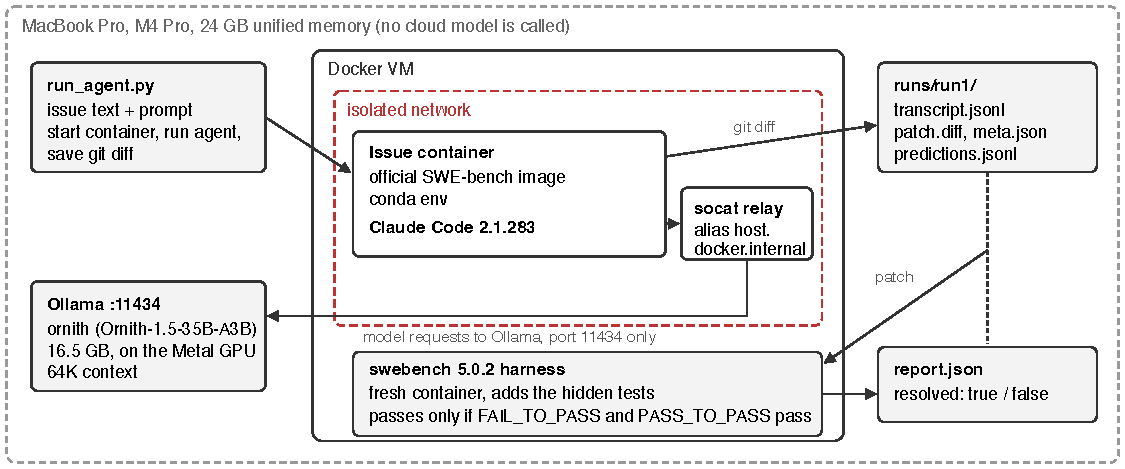
\includegraphics[width=0.97\textwidth]{architecture.pdf}
 \end{center}
 \vspace{-6pt}
 \resumeItemListStart
    \resumeItem{Ollama 0.34 serves the model through an Anthropic-compatible Messages endpoint, so Claude Code connects to it via \code{ANTHROPIC\_BASE\_URL}. For each issue, \code{run\_agent.py} starts the issue's official SWE-bench image, which holds the repository at \code{/testbed} on the issue's base commit plus a conda environment where Django's tests run. The runner mounts a Linux Claude Code binary and runs it headless with the issue text as the prompt. When the agent stops, the runner saves \code{git diff} (excluding \code{tests/}) with the transcript and per-issue statistics. The \code{swebench} harness then applies each patch in a fresh container, adds the hidden tests, and marks the issue resolved only if the new tests (FAIL\_TO\_PASS) pass and the existing ones (PASS\_TO\_PASS) still pass.}
 \resumeItemListEnd

%-----------DESIGN DECISIONS-----------
\section{Design Decisions}
 \resumeItemListStart
    \resumeItem{\textbf{The agent runs inside the task container.} The container has the right Python and dependencies, so the agent can run Django's tests, and it is the sandbox so the agent can do any action freely without the risk of doing something malicious on the system.}
    \resumeItem{\textbf{The agent has no internet.} Agent containers sit on an internal Docker network that has no internet access. I added this mid run, after the agent on an issue ran \code{pip download django==3.0} ``to find the actual upstream fix'' rather than fixing it itself. The download timed out, and I discarded that attempt and reran the issue isolated.}
    \resumeItem{\textbf{A seed chose the issues.} I sampled 10 from the 16 Django 3.0 issues labelled ``$<$15 min fix''. After 7 of those 10 were resolved, I tried the rest of the pool and stopped at 10 resolved.}
 \resumeItemListEnd

%-----------RESULTS-----------
\needspace{14\baselineskip}
\section{Results}
 \vspace{4pt}
 {\small
 \setlength{\tabcolsep}{5pt}
 \begin{tabularx}{\textwidth}{@{}>{\raggedright\arraybackslash}Xccccc@{}}
   \toprule
   \textbf{Issue} & \textbf{Resolved} & \textbf{Hidden tests} & \textbf{Existing tests} & \textbf{Minutes} & \textbf{Turns} \\
   \midrule
   10880 DISTINCT with a condition        & yes         & 1/1 & 55/55   & 3.1  & 21 \\
   10914 default upload permissions       & yes         & 1/1 & 98/98   & 3.5  & 28 \\
   10999 negative durations               & \textbf{no} & 0/2 & 10/10   & 6.1  & 19 \\
   11066 content type saved to wrong DB   & yes         & 1/1 & 3/3     & 1.5  & 7  \\
   11099 trailing newline in usernames    & yes         & 3/3 & 19/19   & 1.7  & 15 \\
   11179 delete() keeps the PK            & yes         & 1/1 & 40/40   & 3.0  & 19 \\
   11433 cleaned\_data vs model defaults  & \textbf{no} & 0/1 & 138/142 & 18.3 & 43 \\
   11451 authenticate() with no password  & \textbf{no} & 0/6 & 45/45   & 4.6  & 26 \\
   11490 values() on combined queries     & yes         & 1/1 & 23/23   & 11.7 & 43 \\
   11603 DISTINCT for Avg and Sum         & yes         & 2/2 & 58/58   & 5.6  & 36 \\
   11239 Postgres client certificates     & yes         & 1/1 & 5/5     & 3.4  & 16 \\
   11133 memoryview in HttpResponse       & yes         & 1/1 & 64/64   & 5.7  & 22 \\
   11163 model\_to\_dict(fields=[])       & yes         & 1/1 & 141/141 & 1.8  & 17 \\
   \bottomrule
 \end{tabularx}
 }
 \vspace{2pt}
 \resumeItemListStart
    \resumeItem{The first 10 issues, fixed before any run, gave 7 of 10, and the three extras all resolved. The agent spent 70 minutes on all 13, a median of 3.5 minutes per issue.}
 \resumeItemListEnd

%-----------ANALYSIS-----------
\section{Analysis}
 \resumeItemListStart
    \resumeItem{\textbf{Every run followed the same loop.} The agent found the code, read it, reproduced the bug with a short script, edited, and ran Django's test suite, 2 to 11 times per issue. No run edited a test file or ended with an empty patch. In the five resolved issues I compared line by line with Django's own fix, the agent changed the same line in the same or an equivalent way.}
    \resumeItem{\textbf{All three failures fixed the example and missed a neighbouring case.} On 10999 (the issue of negative durations) the agent applied the one-line regex change the issue text suggests, while Django's fix moves the sign into its own group, so the tests for negative and PostgreSQL-style durations still failed. On 11451 (the authenticate with no password issue) it returns early when the username is missing but still queries the database when the password is missing, so all 6 hidden tests fail. On 11433 (the cleaned\_data vs model defaults) it deleted the check that keeps model defaults instead of narrowing it, which broke 4 existing tests. The agent saw those failures in its own test runs and dismissed them as ``old behavior we're intentionally changing''. That run was also the only one past the 64K context (67K tokens). Failed runs took longer (median 6.1 minutes against 3.2) and used more context (mean largest prompt 43K tokens against 28K).}
    \resumeItem{\textbf{The agent tried to look up answers.} Nothing in the prompt suggested it, yet on 11433 (the issue of cleaned\_data vs model defaults) the agent tried twice to fetch the upstream fix: \code{pip download django==3.0}. Without network isolation, a score from this setup could include copied fixes i.e.\ the agent would have just updated the django version without actually writing any code.}
    \resumeItem{\textbf{Memory of the machine was a constraint.} The model (17\,GB) and Docker's VM (8\,GB) together exceed 24\,GB, and macOS swapped up to 18.9\,GB. Swap cost speed but changed no result.}
    \resumeItem{\textbf{Limitations.} Thirteen easy issues from one repository are a small sample to test the performance of the model comprehensively. Each issue got one attempt at temperature 1.0, so reruns could differ. The model ran at about 3.8 bits per weight in a different harness than the one which gave the 79\% score, so the two numbers are not directly comparable.}
    \resumeItem{\textbf{Code:} \code{runner/} (runner, grading, summary), \code{bin/claude-local} (host launcher), \code{runs/run1/} (transcripts, patches, results), \code{logs/run\_evaluation/} (harness reports).}
 \resumeItemListEnd

%-------------------------------------------
\end{document}
